\section{Funciones Vectoriales}

Una función vectorial generaliza el concepto de función real: en lugar de asignar un número real a cada valor del parámetro, asigna un \textbf{vector}. Son la herramienta fundamental para describir curvas y trayectorias en el espacio, y conectan el cálculo univariable con el análisis multivariable.

\subsection{Definición y Dominio}

\begin{mydefinition}{Función vectorial}
Una función vectorial en $\mathbb{R}^n$ es una función $\vec{r}: D \subseteq \mathbb{R} \to \mathbb{R}^n$ que asigna a cada escalar $t \in D$ un único vector en $\mathbb{R}^n$:
\[ \vec{r}(t) = \bigl(f_1(t),\; f_2(t),\; \dots,\; f_n(t)\bigr) = f_1(t)\,\hat{\imath}_1 + f_2(t)\,\hat{\imath}_2 + \dots + f_n(t)\,\hat{\imath}_n \]
Las funciones reales $f_1, f_2, \dots, f_n$ se llaman funciones componentes de $\vec{r}$.
\end{mydefinition}

El dominio natural de $\vec{r}$ es la intersección de los dominios de sus componentes:
\[ D = \bigcap_{i=1}^{n} \text{Dom}(f_i) \]

\subsection{Límites y Continuidad}

Los conceptos de límite y continuidad se trasladan de manera directa a las funciones vectoriales, operando componente a componente.

\begin{mydefinition}{Límite de una función vectorial}
Si $\vec{r}(t) = (f_1(t), f_2(t), \dots, f_n(t))$, el límite cuando $t \to a$ se define como:
\[ \lim_{t \to a} \vec{r}(t) = \left(\lim_{t \to a} f_1(t),\; \lim_{t \to a} f_2(t),\; \dots,\; \lim_{t \to a} f_n(t)\right) \]
siempre que los límites escalares existan.
\end{mydefinition}

\begin{mydefinition}{Continuidad}
Una función vectorial $\vec{r}(t)$ es continua en $t = a$ si:
\[ \lim_{t \to a} \vec{r}(t) = \vec{r}(a) \]
Esto ocurre si y solo si cada función componente es continua en $t = a$.
\end{mydefinition}

La continuidad de $\vec{r}(t)$ en su dominio garantiza que la curva trazada en el espacio no tiene saltos ni discontinuidades: es una curva \textit{suave por partes}.


\subsection{Representación Gráfica}

La imagen geométrica de una función vectorial $\vec{r}(t)$, conforme $t$ recorre su dominio, es una curva en $\mathbb{R}^n$. Cada valor de $t$ determina la posición de un punto sobre dicha curva.

\subsubsection{Curvas planas en $\mathbb{R}^2$}

Si la componente $z$ es cero, la curva yace en el plano $xy$. Por ejemplo, sea: $\vec{r}(t) = (\cos t, \sin t, 0)$ con $t \in [0, 2\pi]$ traza el círculo unitario.

\begin{center}
\shorthandoff{>}
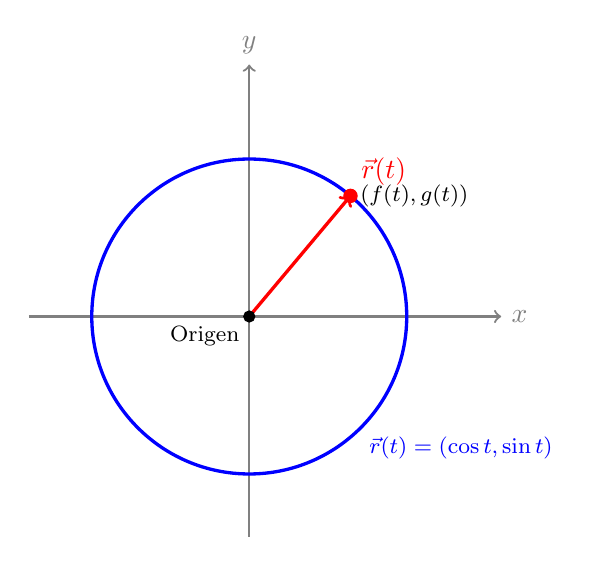
\begin{tikzpicture}[scale=2]
    \draw[->, gray, thick] (-1.4,0) -- (1.6,0) node[right] {$x$};
    \draw[->, gray, thick] (0,-1.4) -- (0,1.6) node[above] {$y$};

    \draw[very thick, blue] (1,0) arc (0:360:1);

    \draw[->, very thick, red] (0,0) -- ({cos(50)},{sin(50)}) node[above right] {$\vec{r}(t)$};

    \filldraw[red] ({cos(50)},{sin(50)}) circle (1.2pt);
    \node[right, font=\footnotesize] at ({cos(50)},{sin(50)}) {$(f(t), g(t))$};

    \node[below right, blue, font=\footnotesize] at (0.7,-0.7) {$\vec{r}(t) = (\cos t, \sin t)$};
    \filldraw[black] (0,0) circle (1pt) node[below left] {\footnotesize Origen};
\end{tikzpicture}
\end{center}

\subsubsection{La hélice circular en $\mathbb{R}^3$}

Uno de los ejemplos más representativos de curva en el espacio es la hélice circular:
\[ \vec{r}(t) = (a\cos t,\; a\sin t,\; bt), \quad t \in \mathbb{R} \]
donde $a$ controla el radio y $b$ el paso. Las proyecciones sobre el plano $xy$ forman un círculo, mientras que la curva asciende de forma uniforme.

\begin{center}
\shorthandoff{>}
\begin{tikzpicture}[x={(-0.5cm,-0.4cm)}, y={(1cm,0cm)}, z={(0cm,1cm)}, scale=1.8]
    \draw[->, gray, thick] (0,0,0) -- (2,0,0) node[below left] {$x$};
    \draw[->, gray, thick] (0,0,0) -- (0,2,0) node[right] {$y$};
    \draw[->, gray, thick] (0,0,0) -- (0,0,2.8) node[above] {$z$};

    \draw[very thick, blue, variable=\t, domain=0:360, samples=36, smooth]
        plot ({cos(\t)}, {sin(\t)}, {\t/360});
    \draw[very thick, blue, variable=\t, domain=360:720, samples=36, smooth]
        plot ({cos(\t)}, {sin(\t)}, {\t/360});

    \draw[dashed, gray, variable=\t, domain=0:360, samples=24, smooth]
        plot ({cos(\t)}, {sin(\t)}, 0);

    \draw[dashed, gray!50] (1,0,0) -- (1,0,2);

    \filldraw[red] ({cos(90)},{sin(90)},{0.25}) circle (1.5pt)
        node[right=2pt, black, font=\footnotesize] {$\vec{r}(t_0)$};

    \node[blue, font=\footnotesize] at (-2.0,-0.1,2.5)
        {$\vec{r}(t)=(\cos t,\,\sin t,\,\tfrac{t}{2\pi})$};
\end{tikzpicture}
\end{center}

\subsection{Derivadas de Funciones Vectoriales}

\begin{mydefinition}{Derivada de una función vectorial}
La derivada de $\vec{r}(t)$ se define de manera análoga a la derivada escalar:
\[ \vec{r}'(t) = \lim_{\Delta t \to 0} \frac{\vec{r}(t + \Delta t) - \vec{r}(t)}{\Delta t} \]
Si $\vec{r}(t) = (f_1(t), f_2(t), \dots ,f_n(t))$, entonces:
\[ \vec{r}'(t) = \bigl(f_1'(t),\; f_2'(t),\; \dots ,\; f_n'(t)\bigr) \]
siempre que las $n$ derivadas componentes existan. En ese caso se dice que $\vec{r}$ es \textbf{diferenciable} en $t$.
\end{mydefinition}

\subsubsection{Interpretación geométrica}

El vector $\vec{r}(t + \Delta t) - \vec{r}(t)$ une dos puntos de la curva. Al dividirlo entre $\Delta t$ y tomar el límite, se obtiene un vector que es tangente a la curva en el punto $\vec{r}(t)$, apuntando en la dirección del movimiento.

\begin{center}
\shorthandoff{>}
\begin{tikzpicture}[scale=1.4]
    \draw[->, gray] (-0.5,0) -- (4.5,0) node[right] {$x$};
    \draw[->, gray] (0,-0.5) -- (0,3) node[above] {$y$};

    \draw[very thick, blue, domain=0.2:3.8, samples=80]
        plot (\x, {0.4*\x*\x - 0.5*\x + 1.2});

    \coordinate (P) at (2, {0.4*4 - 1 + 1.2});
    \coordinate (Q) at (3, {0.4*9 - 1.5 + 1.2});

    \draw[->, very thick, purple] (P) -- (Q) node[midway, above left, font=\footnotesize] {$\vec{r}(t{+}\Delta t) - \vec{r}(t)$};

    \draw[->, very thick, red] (P) -- ++(1, {2*0.4*2 - 0.5}) node[right] {$\vec{r}'(t)$};

    \filldraw[black] (P) circle (1.5pt) node[below left] {$\vec{r}(t)$};
    \filldraw[black] (Q) circle (1.5pt) node[above right] {$\vec{r}(t{+}\Delta t)$};
\end{tikzpicture}
\end{center}

\subsubsection{Reglas de derivación}

\begin{mytheorem}{Reglas de derivación vectorial}
Sean $\vec{u}(t)$ y $\vec{v}(t)$ funciones vectoriales diferenciables y $c(t)$ una función escalar diferenciable. Entonces:
\begin{enumerate}
    \item $\dfrac{d}{dt}[\vec{u} + \vec{v}] = \vec{u}' + \vec{v}'$
    \item $\dfrac{d}{dt}[c\,\vec{u}] = c'\vec{u} + c\,\vec{u}'$
    \item $\dfrac{d}{dt}[\vec{u} \cdot \vec{v}] = \vec{u}' \cdot \vec{v} + \vec{u} \cdot \vec{v}'$
    \item $\dfrac{d}{dt}[\vec{u} \times \vec{v}] = \vec{u}' \times \vec{v} + \vec{u} \times \vec{v}'$
    \item $\dfrac{d}{dt}[\vec{u}(c(t))] = c'(t)\,\vec{u}'(c(t))$ \quad (Regla de la cadena)
\end{enumerate}
\end{mytheorem}
    
\subsection{Integrales de Funciones Vectoriales}

La integral de una función vectorial también se aplica componente a componente.

\begin{mydefinition}{Integral indefinida}
\[ \int \vec{r}(t)\, dt = \left(\int f_1(t)\,dt,\; \int f_2(t)\,dt,\; \dots ,\; \int f_n(t)\,dt\right) + \vec{C} \]
donde $\vec{C} = (C_1, C_2, \dots , C_n)$ es un \textbf{vector constante de integración}.
\end{mydefinition}

\begin{mydefinition}{Integral definida}
\[ \int_a^b \vec{r}(t)\, dt = \left(\int_a^b f_1(t)\,dt,\; \int_a^b f_2(t)\,dt,\; \dots ,\; \int_a^b f_n(t)\,dt\right) \]
\end{mydefinition}

El Teorema Fundamental del Cálculo también aplica: si $\vec{R}(t)$ es una antiderivada de $\vec{r}(t)$, es decir, $\vec{R}'(t) = \vec{r}(t)$, entonces:
\[ \int_a^b \vec{r}(t)\, dt = \vec{R}(b) - \vec{R}(a) \]

\subsection{Cinemática Vectorial}

La aplicación más natural de las funciones vectoriales es la descripción del movimiento de una partícula en el espacio. Si $\vec{r}(t)$ representa la \textbf{posición} de la partícula en el instante $t$, las sucesivas derivadas codifican cantidades cinemáticas con significado físico preciso.

\subsubsection{Posición, velocidad y aceleración}

\begin{mydefinition}{Cantidades cinemáticas}
Sea $\vec{r}(t) = (x(t), y(t), z(t))$ la función de posición de una partícula. Se definen:
\begin{itemize}
    \item \textbf{Vector velocidad:} $\vec{v}(t) = \vec{r}'(t) = \bigl(x'(t),\, y'(t),\, z'(t)\bigr)$
    \item \textbf{Rapidez escalar:} $v(t) = \|\vec{v}(t)\| = \|\vec{r}'(t)\|$
    \item \textbf{Vector aceleración:} $\vec{a}(t) = \vec{v}'(t) = \vec{r}''(t) = \bigl(x''(t),\, y''(t),\, z''(t)\bigr)$
\end{itemize}
\end{mydefinition}

Una propiedad importante de la cinemática vectorial es que el vector velocidad es siempre tangente a la trayectoria. Por definición de derivada, el vector $\vec{r}(t + \Delta t) - \vec{r}(t)$ une dos posiciones cercanas de la partícula. Al dividir entre $\Delta t$ y tomar el límite, el resultado apunta exactamente en la dirección en que la curva avanza en ese instante. Por lo tanto, $\vec{v}(t)$ es tangente a la curva y su módulo es la rapidez con la que la partícula la recorre.

\begin{center}
\shorthandoff{>}
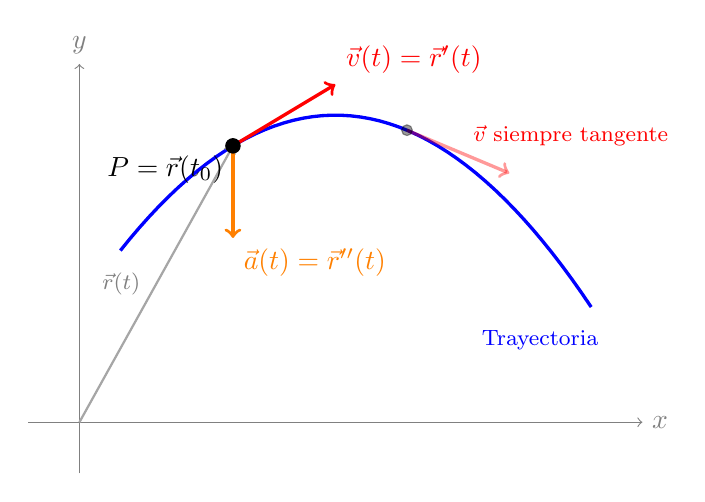
\begin{tikzpicture}[scale=1.3]
    \draw[->, gray] (-0.5,0) -- (5.5,0) node[right] {$x$};
    \draw[->, gray] (0,-0.5) -- (0,3.5) node[above] {$y$};

    % Trayectoria (parábola orientada)
    \draw[very thick, blue, domain=0.4:5, samples=50]
        plot (\x, {-0.3*(\x-2.5)*(\x-2.5) + 3});

    % Punto en t=t0 (x=1.5)
    \def\px{1.5}
    \def\py{-0.3*(1.5-2.5)*(1.5-2.5)+3}  % = -0.3 + 3 = 2.7

    % Vector posición
    \draw[->, thick, gray!70] (0,0) -- (\px, 2.7) node[midway, left=2pt, font=\footnotesize, gray] {$\vec{r}(t)$};

    % Derivada de la parábola: y' = -0.6(x-2.5), en x=1.5: y' = -0.6*(-1) = 0.6
    % Vector velocidad (tangente): dirección (1, 0.6), normalizado para visual
    \draw[->, very thick, red] (\px, 2.7) -- ++(1.0, 0.6) node[above right] {$\vec{v}(t) = \vec{r}'(t)$};

    % Vector aceleración (2ª derivada, apunta hacia abajo: y''=-0.6)
    \draw[->, very thick, orange] (\px, 2.7) -- ++(0, -0.9) node[below right] {$\vec{a}(t) = \vec{r}''(t)$};

    % Punto
    \filldraw[black] (\px, 2.7) circle (2pt) node[below left] {$P = \vec{r}(t_0)$};

    % Punto futuro
    \def\px2{3.2}
    \draw[->, very thick, red, opacity=0.4] (\px2, {-0.3*(\px2-2.5)*(\px2-2.5)+3}) -- ++(1.0, {-0.6*(\px2-2.5)}) ;
    \filldraw[black, opacity=0.4] (\px2, {-0.3*(\px2-2.5)*(\px2-2.5)+3}) circle (1.5pt);

    \node[blue, font=\footnotesize] at (4.5, 0.8) {Trayectoria};
    \node[font=\footnotesize, align=left] at (4.8, 2.8) {\textcolor{red}{$\vec{v}$ siempre tangente}};
\end{tikzpicture}
\end{center}

La aceleración $\vec{a}(t)$ mide cómo cambia el \textit{vector} velocidad, no solo su magnitud. Esto tiene una consecuencia importante: una partícula puede tener aceleración no nula aunque su rapidez sea constante, simplemente porque está cambiando de dirección.

El caso más ilustrativo es el movimiento circular uniforme: Sea $\vec{r}(t) = (R\cos t,\; R\sin t)$, con radio $R$ y velocidad angular constante $1$ rad/s.
\begin{align*}
    \vec{v}(t) &= (-R\sin t,\; R\cos t) & \|\vec{v}(t)\| &= R \quad \text{(rapidez constante)} \\
    \vec{a}(t) &= (-R\cos t,\; -R\sin t) = -\vec{r}(t) & \|\vec{a}(t)\| &= R
\end{align*}

\begin{center}
\shorthandoff{>}
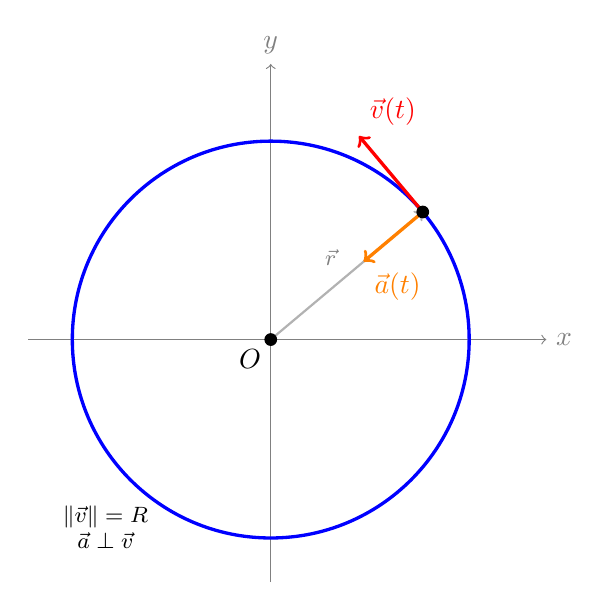
\begin{tikzpicture}[scale=1.4]
    \draw[->, gray] (-2.2,0) -- (2.5,0) node[right] {$x$};
    \draw[->, gray] (0,-2.2) -- (0,2.5) node[above] {$y$};

    % Círculo
    \draw[very thick, blue] (0,0) circle (1.8cm);

    % Punto en t=40 grados
    \def\ang{40}
    \def\R{1.8}
    \coordinate (P) at ({1.8*cos(\ang)}, {1.8*sin(\ang)});

    % Vector posición
    \draw[->, thick, gray!60] (0,0) -- (P) node[midway, above left, font=\footnotesize, gray] {$\vec{r}$};

    % Vector velocidad (tangente al círculo: dirección (-sin, cos))
    \draw[->, very thick, red] (P) -- ++({-\R*0.5*sin(\ang)}, {\R*0.5*cos(\ang)})
        node[above right] {$\vec{v}(t)$};

    % Vector aceleración (centrípeta: apunta hacia el centro)
    \draw[->, very thick, orange] (P) -- ++({-0.7*cos(\ang)}, {-0.7*sin(\ang)})
        node[below right] {$\vec{a}(t)$};

    \filldraw[black] (P) circle (1.5pt);
    \filldraw[black] (0,0) circle (1.5pt) node[below left] {$O$};

    \node[font=\footnotesize, align=center] at (-1.5,-1.7)
        {$\|\vec{v}\| = R$ \\$\vec{a} \perp \vec{v}$};
\end{tikzpicture}
\end{center}

La aceleración $\vec{a} = -\vec{r}$ apunta siempre hacia el centro del círculo (aceleración centrípeta), y es perpendicular a la velocidad en todo momento: $\vec{v} \cdot \vec{a} = 0$.

Por otro lado, dado que $\vec{v}(t) = \vec{r}'(t)$, se puede recuperar la posición integrando si se conoce la condición inicial:
\[ \vec{r}(t) = \vec{r}(t_0) + \int_{t_0}^{t} \vec{v}(u)\, du \]
De manera análoga, conociendo $\vec{a}(t)$ y las condiciones iniciales $\vec{v}(t_0)$ y $\vec{r}(t_0)$, se puede reconstruir toda la trayectoria.

Utilizando el ejemplo de un proyectil: Una pelota se lanza con velocidad inicial $\vec{v}_0 = (v_0\cos\alpha,\; v_0\sin\alpha)$ desde el origen. La única aceleración es la gravedad: $\vec{a}(t) = (0, -g)$.

Integrando una vez: $\vec{v}(t) = \vec{v}_0 + \int_0^t \vec{a}\, du = (v_0\cos\alpha,\; v_0\sin\alpha - gt)$.

Integrando de nuevo con $\vec{r}(0) = \vec{0}$:
\[ \vec{r}(t) = \left(v_0\cos\alpha\cdot t,\;\; v_0\sin\alpha\cdot t - \tfrac{1}{2}g t^2\right) \]

\begin{center}
\shorthandoff{>}
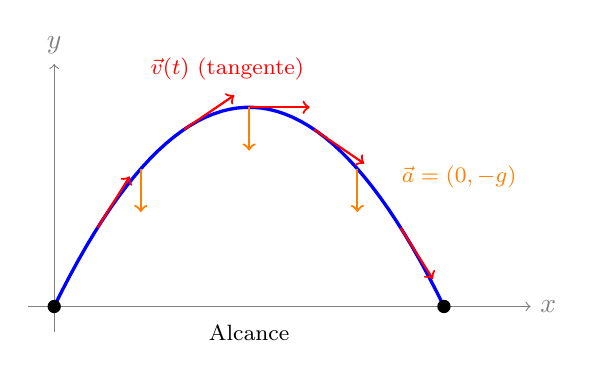
\begin{tikzpicture}[scale=1.1]
    \draw[->, gray] (-0.3,0) -- (5.5,0) node[right] {$x$};
    \draw[->, gray] (0,-0.3) -- (0,2.8) node[above] {$y$};

    % Parábola con v0=5, alpha=45, g=9.8: x=5cos45*t, y=5sin45*t - 4.9t^2
    % max height at t=5sin45/9.8 ≈ 0.361 s: y≈0.638
    % range at t=2*0.361≈0.722 s: x≈2.552
    % Scale so it looks good: multiply t by 1, scale x by 2
    % r(t) = (5cos45*t, 5sin45*t - 4.9t^2), t in [0, 0.722]
    % Scale x by 2 visually -> (3.536t*2, 3.536t - 4.9t^2) = (7.07t, 3.536t - 4.9t^2)
    % Let's parametrize with domain for nice plot: scale everything
    % Use: x = t, y = t*(1-t/T)*H where T=4.5, H=2.3
    \draw[very thick, blue, domain=0:4.5, samples=50]
        plot (\x, {2.3*(\x/4.5)*(1 - \x/4.5)*4});

    % Velocity vectors at a few points
    % dy/dx = 2.3*(1/4.5)*(1 - 2*x/(4.5))*4 = (2.3*4/4.5)*(1-2x/4.5)
    \foreach \xp/\sc in {0.5/0.5, 1.5/0.45, 2.25/0.4, 3.0/0.45, 4.0/0.5} {
        \pgfmathsetmacro{\yp}{2.3*(\xp/4.5)*(1-\xp/4.5)*4}
        \pgfmathsetmacro{\slope}{(2.3*4/4.5)*(1-2*\xp/4.5)}
        \pgfmathsetmacro{\norm}{sqrt(1+\slope*\slope)}
        \draw[->, red, thick]
            (\xp, \yp) -- ++({0.7/\norm}, {0.7*\slope/\norm});
    }

    % Gravity arrows
    \foreach \xp in {1.0, 2.25, 3.5} {
        \pgfmathsetmacro{\yp}{2.3*(\xp/4.5)*(1-\xp/4.5)*4}
        \draw[->, orange, thick] (\xp, \yp) -- ++(0, -0.5) node[right, font=\tiny] {};
    }

    \filldraw[black] (0,0) circle (2pt);
    \filldraw[black] (4.5,0) circle (2pt);

    \node[above right, red, font=\footnotesize] at (1.0, 2.5) {$\vec{v}(t)$ (tangente)};
    \node[right, orange, font=\footnotesize] at (3.9, 1.5) {$\vec{a} = (0,-g)$};
    \node[font=\footnotesize] at (2.25, -0.3) {Alcance};
\end{tikzpicture}
\end{center}

\subsubsection{Longitud de arco}

Intuitivamente, la longitud de una curva es el resultado de ``enderezarla''. Para calcularla de forma rigurosa, se utiliza el mismo principio que en el cálculo integral: aproximar con objetos sencillos (segmentos de recta) y tomar un límite.

Dividiendo el intervalo $[a, b]$ en $n$ subintervalos iguales mediante los puntos $a = t_0 < t_1 < \cdots < t_n = b$, con paso $\Delta t = \frac{b-a}{n}$. Cada $t_i$ define un punto $P_i = \vec{r}(t_i)$ sobre la curva.

Uniendo los puntos consecutivos $P_i$ y $P_{i+1}$ con segmentos de recta, formando una poligonal inscrita en la curva. La longitud del segmento $i$-ésimo es:
\[ \Delta L_i = \|P_{i+1} - P_i\| = \|\vec{r}(t_{i+1}) - \vec{r}(t_i)\| \]

\begin{center}
\shorthandoff{>}
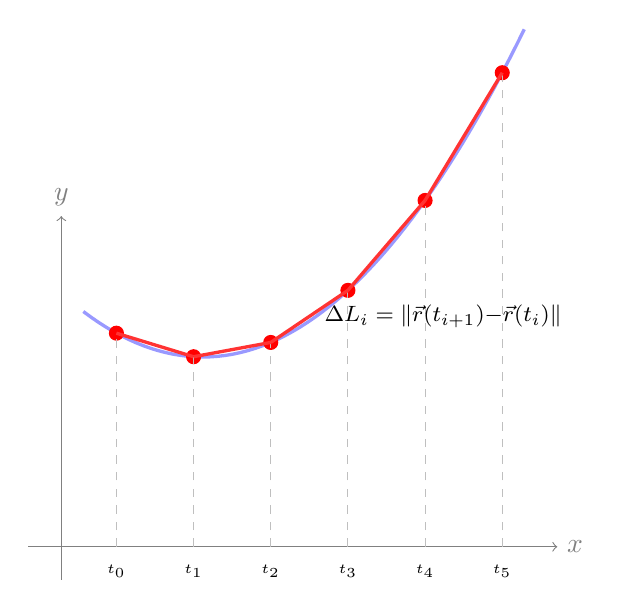
\begin{tikzpicture}[scale=1.4]
    \draw[->, gray] (-0.3,0) -- (4.5,0) node[right] {$x$};
    \draw[->, gray] (0,-0.3) -- (0,3) node[above] {$y$};

    % Curva suave
    \draw[very thick, blue!40, domain=0.2:4.2, samples=60]
        plot (\x, {0.35*\x*\x - 0.9*\x + 2.3});

    % Puntos de la partición
    \foreach \xv/\lab in {0.5/t_0, 1.2/t_1, 1.9/t_2, 2.6/t_3, 3.3/t_4, 4.0/t_5} {
        \pgfmathsetmacro{\yv}{0.35*\xv*\xv - 0.9*\xv + 2.3}
        \filldraw[red] (\xv, \yv) circle (1.8pt);
        \node[font=\tiny, below=3pt] at (\xv, 0) {$\lab$};
        \draw[dashed, gray!50, thin] (\xv, 0) -- (\xv, \yv);
    }

    % Segmentos de la poligonal
    \foreach \xa/\xb in {0.5/1.2, 1.2/1.9, 1.9/2.6, 2.6/3.3, 3.3/4.0} {
        \pgfmathsetmacro{\ya}{0.35*\xa*\xa - 0.9*\xa + 2.3}
        \pgfmathsetmacro{\yb}{0.35*\xb*\xb - 0.9*\xb + 2.3}
        \draw[very thick, red!80] (\xa, \ya) -- (\xb, \yb);
    }

    % Etiqueta de un segmento
    \pgfmathsetmacro{\ymid}{(0.35*1.9*1.9-0.9*1.9+2.3+0.35*2.6*2.6-0.9*2.6+2.3)/2}
    \node[font=\footnotesize, right=2pt] at (2.25, \ymid) {$\Delta L_i = \|\vec{r}(t_{i+1}){-}\vec{r}(t_i)\|$};

\end{tikzpicture}
\end{center}

Por la definición de derivada, cuando $\Delta t$ es pequeño:
\[ \vec{r}(t_i + \Delta t) - \vec{r}(t_i) \approx \vec{r}'(t_i)\,\Delta t \]
Por lo tanto, la longitud de cada cuerda se aproxima por:
\[ \Delta L_i = \|\vec{r}(t_{i+1}) - \vec{r}(t_i)\| \approx \|\vec{r}'(t_i)\|\,\Delta t \]

La siguiente figura ilustra esto geométricamente: al acercar $P_{i+1}$ a $P_i$, la cuerda (roja) es casi indistinguible del vector tangente escalado $\vec{r}'(t_i)\Delta t$ (azul).

\begin{center}
\shorthandoff{>}
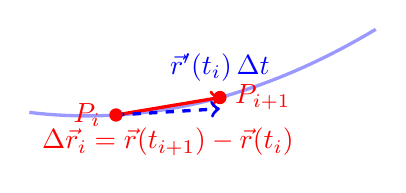
\begin{tikzpicture}[scale=2.2]
    % Arco de curva local
    \draw[very thick, blue!40, domain=0.5:2.5, samples=40]
        plot (\x, {0.18*\x*\x - 0.3*\x + 1.2});

    % Dos puntos cercanos
    \def\xa{1.0}  \def\ya{0.18*1.0*1.0-0.3*1.0+1.2}   % ≈ 1.08
    \def\xb{1.6}  \def\yb{0.18*1.6*1.6-0.3*1.6+1.2}   % ≈ 1.261

    \coordinate (Pi)  at (\xa, {0.18*1.0*1.0-0.3*1.0+1.2});
    \coordinate (Pi1) at (\xb, {0.18*1.6*1.6-0.3*1.6+1.2});

    % Cuerda (Δr)
    \draw[->, very thick, red] (Pi) -- (Pi1)
        node[midway, below=4pt] {$\Delta\vec{r}_i = \vec{r}(t_{i+1})-\vec{r}(t_i)$};

    % Tangente escalada r'(t)*Δt (pendiente en xa: 0.36*1-0.3=0.06, Δx=0.6)
    % Vector tangente real: (1, 0.06), escalar a Δx=0.6
    \draw[->, very thick, blue, dashed] (Pi) -- ++(0.6, 0.036)
        node[above=6pt] {$\vec{r}'(t_i)\,\Delta t$};

    % Puntos
    \filldraw[red] (Pi) circle (1pt) node[left=2pt] {$P_i$};
    \filldraw[red] (Pi1) circle (1pt) node[right=2pt] {$P_{i+1}$};
\end{tikzpicture}
\end{center}

La longitud total de la poligonal es:
\[ L_n = \sum_{i=0}^{n-1} \Delta L_i \approx \sum_{i=0}^{n-1} \|\vec{r}'(t_i)\|\,\Delta t \]
Esta es una suma de Riemann para la función $\|\vec{r}'(t)\|$. Al hacer $n \to \infty$ (equivalente a $\Delta t \to 0$), la poligonal converge a la curva real y la suma converge a la integral:

\begin{mydefinition}{Longitud de arco}
Sea $\vec{r}(t)$ continuamente diferenciable en $[a, b]$. La longitud de arco de la curva es:
\[ L = \lim_{n\to\infty} \sum_{i=0}^{n-1}\|\vec{r}'(t_i)\|\,\Delta t = \int_a^b \|\vec{r}'(t)\|\, dt \]
Expandiendo la norma en sus componentes:
\[ L = \int_a^b \sqrt{\,[x'(t)]^2 + [y'(t)]^2 + [z'(t)]^2}\; dt \]
\end{mydefinition}

\subsubsection{Parámetro de longitud de arco}

Es posible reparametrizar la curva usando como parámetro la longitud de arco $s$ acumulada desde $t = a$:
\[ s(t) = \int_a^t \|\vec{r}'(u)\|\, du \]
Por el Teorema Fundamental del Cálculo, $\dfrac{ds}{dt} = \|\vec{r}'(t)\| = v(t)$. Esto permite cambiar entre los dos parámetros:
\begin{itemize}
    \item $s$ como función de $t$: mide cuánta longitud se ha recorrido hasta el instante $t$.
    \item $t$ como función de $s$: invirtiendo la relación, permite localizar en qué punto de la curva se está habiendo recorrido una distancia $s$.
\end{itemize}

\subsection{Los vectores $\hat{T}$, $\hat{N}$ y $\hat{B}$ de Frenet-Serret}

Para analizar la geometría de una curva en el espacio (sin importar cómo se parametrice), se construye un sistema de referencia móvil asociado a cada punto de la curva: el triedro de Frenet-Serret, formado por tres vectores unitarios y mutuamente ortogonales $\hat{T}$, $\hat{N}$ y $\hat{B}$.

\begin{center}
\shorthandoff{>}
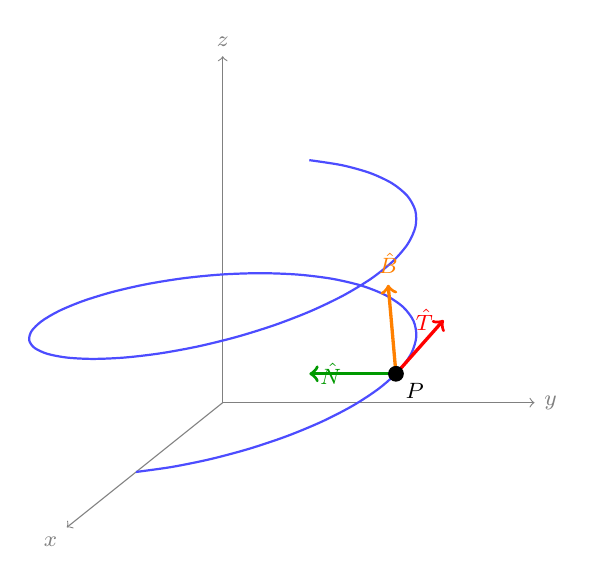
\begin{tikzpicture}[x={(-0.5cm,-0.4cm)}, y={(1cm,0cm)}, z={(0cm,1cm)}, scale=2.2]
    \draw[->, gray] (0,0,0) -- (1.8,0,0) node[below left, font=\footnotesize] {$x$};
    \draw[->, gray] (0,0,0) -- (0,1.8,0) node[right, font=\footnotesize] {$y$};
    \draw[->, gray] (0,0,0) -- (0,0,2.0) node[above, font=\footnotesize] {$z$};

    % Hélice r(t)=(cos t, sin t, t/360) para t en grados, una vuelta y media
    \draw[thick, blue!70, variable=\t, domain=0:540, samples=48, smooth]
        plot ({cos(\t)}, {sin(\t)}, {\t/540});

    % Punto en t=90 grados: P=(0, 1, 90/540) = (0, 1, 1/6)
    % T = (-1, 0, ~0.16) normalizado ≈ (-0.988, 0, 0.157)
    % N = (0, -1, 0)
    % B = T x N ≈ (0.157, 0, 0.988)
    \coordinate (P) at ({cos(90)}, {sin(90)}, {90/540});

    \draw[->, very thick, red]         (P) -- ++(-0.55, 0,    0.09) node[left, font=\footnotesize] {$\hat{T}$};
    \draw[->, very thick, green!60!black] (P) -- ++(0,   -0.5, 0)    node[right, font=\footnotesize] {$\hat{N}$};
    \draw[->, very thick, orange]      (P) -- ++(0.09,  0,    0.55) node[above, font=\footnotesize] {$\hat{B}$};

    \filldraw[black] (P) circle (1.2pt) node[below right, font=\footnotesize] {$P$};
\end{tikzpicture}
\end{center}

\begin{center}
{\footnotesize
\begin{tabular}{ccc}
    \textcolor{red}{$\hat{T}$: tangente (dirección de movimiento)} &
    \textcolor{green!60!black}{$\hat{N}$: normal principal (hacia donde dobla)} &
    \textcolor{orange}{$\hat{B}$: binormal ($\hat{T}\times\hat{N}$)}
\end{tabular}
}
\end{center}

\subsubsection{Vector tangente unitario $\hat{T}$}

El vector tangente unitario apunta en la dirección del movimiento y se obtiene normalizando la derivada de la posición:

\begin{mydefinition}{Vector tangente unitario}
\[ \hat{T}(t) = \frac{\vec{r}'(t)}{\|\vec{r}'(t)\|} \]
\end{mydefinition}

\subsubsection{Curvatura $\kappa$}

La curvatura mide cuánto cambia la dirección de la curva por unidad de longitud de arco, es decir, qué tan rápido se dobla la curva.

\begin{mydefinition}{Curvatura}
La curvatura $\kappa$ de una curva en $\mathbb{R}^3$ se define como:
\[ \kappa = \left\|\frac{d\hat{T}}{ds}\right\| = \frac{\|\hat{T}'(t)\|}{\|\vec{r}'(t)\|} \]
Una fórmula alternativa, más práctica para el cálculo, es:
\[ \kappa = \frac{\|\vec{r}'(t) \times \vec{r}''(t)\|}{\|\vec{r}'(t)\|^3} \]
\end{mydefinition}


\subsubsection{Vector normal principal $\hat{N}$}

El vector normal principal apunta hacia el interior de la curva. Este vector se obtiene normalizando la derivada del vector tangente unitario. Dado que $\hat{T}$ es unitario, su derivada es siempre perpendicular a $\hat{T}$, lo que garantiza que $\hat{N}$ también es perpendicular a $\hat{T}$.

\begin{mydefinition}{Vector normal principal}
\[ \hat{N}(t) = \frac{\hat{T}'(t)}{\|\hat{T}'(t)\|} \]
\end{mydefinition}

\subsubsection{Vector binormal $\hat{B}$}

El vector binormal completa el triedro de Frenet-Serret como un tercer vector ortogonal a los dos anteriores. Es el producto vectorial de $\hat{T}$ y $\hat{N}$, y apunta en la dirección perpendicular al plano osculador formado por $\hat{T}$ y $\hat{N}$.

\begin{mydefinition}{Vector binormal}
\[ \hat{B}(t) = \hat{T}(t) \times \hat{N}(t) \]
\end{mydefinition}

El plano determinado por $\hat{N}$ y $\hat{B}$ se llama plano normal, y el plano determinado por $\hat{T}$ y $\hat{B}$ se llama plano rectificante.

\subsubsection{Resumen del triedro de Frenet-Serret}

\begin{mytheorem}{Fórmulas de Frenet-Serret}
Los tres vectores del triedro satisfacen las siguientes relaciones diferenciales:
\[
\frac{d\hat{T}}{ds} = \kappa\,\hat{N}, \qquad
\frac{d\hat{N}}{ds} = -\kappa\,\hat{T} + \tau\,\hat{B}, \qquad
\frac{d\hat{B}}{ds} = -\tau\,\hat{N}
\]
donde $\kappa \geq 0$ es la curvatura y $\tau$ es la torsión.
\end{mytheorem}

\subsubsection{Descomposición de la aceleración}

Una consecuencia importante del triedro de Frenet-Serret es que la aceleración siempre yace en el plano osculador y se puede descomponer en dos componentes ortogonales:

\begin{mytheorem}{Componentes tangencial y normal de la aceleración}
\[ \vec{a}(t) = a_T\,\hat{T} + a_N\,\hat{N} \]
donde:
\[ a_T = \frac{d^2s}{dt^2} = \frac{\vec{r}'(t) \cdot \vec{r}''(t)}{\|\vec{r}'(t)\|} \qquad \text{(componente tangencial)} \]
\[ a_N = \kappa \left(\frac{ds}{dt}\right)^2 = \frac{\|\vec{r}'(t) \times \vec{r}''(t)\|}{\|\vec{r}'(t)\|} \qquad \text{(componente normal)} \]
La componente $a_T$ refleja el cambio de rapidez; la componente $a_N$ refleja el cambio de dirección.
\end{mytheorem}

\begin{center}
\shorthandoff{>}
% Curva: y = 0.5 + 0.7*sin(70*x)  [angulo en grados]
% Punto P en x=1.0:
%   y(1)  = 0.5 + 0.7*sin(70°)  ≈ 1.158
%   y'(1) = 0.7*cos(70°)*(70π/180) ≈ 0.292   →  T̂ ≈ (0.960, 0.280)
%   y''(1) < 0  (concava hacia abajo)         →  N̂ ≈ (0.280, -0.960)
% Componentes elegidas: a_T = 0.7, a_N = 0.5
%   a_T·T̂ ≈ (0.672,  0.196)
%   a_N·N̂ ≈ (0.140, -0.480)
%   a     ≈ (0.812, -0.284)   [suma exacta → paralelogramo cierra]
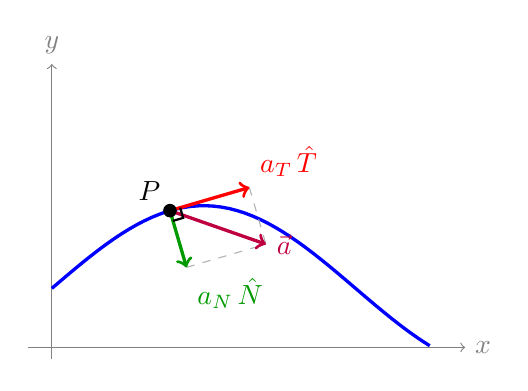
\begin{tikzpicture}[scale=1.5]
    \draw[->, gray, thin] (-0.2,0) -- (3.5,0) node[right] {$x$};
    \draw[->, gray, thin] (0,-0.1) -- (0,2.4) node[above] {$y$};

    \draw[very thick, blue, domain=0:3.2, samples=50]
        plot (\x, {0.5 + 0.7*sin(70*\x)});

    \coordinate (P)  at (1.0,   1.158);   % punto base
    \coordinate (AT) at (1.672, 1.354);   % P + a_T·T̂
    \coordinate (AN) at (1.140, 0.678);   % P + a_N·N̂
    \coordinate (A)  at (1.812, 0.874);   % P + a  (= AT + a_N·N̂ = AN + a_T·T̂)

    % Paralelogramo (líneas punteadas)
    \draw[dashed, gray!60, thin] (AT) -- (A);
    \draw[dashed, gray!60, thin] (AN) -- (A);

    % Aceleración total
    \draw[->, very thick, purple] (P) -- (A)
        node[right] {$\vec{a}$};

    % Componente tangencial (a lo largo de T̂, paralela a la curva)
    \draw[->, very thick, red] (P) -- (AT)
        node[above right] {$a_T\,\hat{T}$};

    % Componente normal (perpendicular a T̂, hacia el centro de curvatura)
    \draw[->, very thick, green!60!black] (P) -- (AN)
        node[below right] {$a_N\,\hat{N}$};

    % Marca de ángulo recto en P entre T̂ y N̂
    % paso ε=0.09 a lo largo de T̂=(0.960,0.280) y N̂=(0.280,-0.960)
    \draw[thick]
        (1.0864, 1.1832)            % P + ε·T̂
        -- (1.1116, 1.0968)         % P + ε·T̂ + ε·N̂
        -- (1.0252, 1.0716);        % P + ε·N̂

    \filldraw[black] (P) circle (1.5pt) node[above left] {$P$};
\end{tikzpicture}
\end{center}

\subsection{Ejercicios}

\begin{enumerate}
    \item Determinar el dominio natural de cada función vectorial:
\begin{enumerate}
    \item $\vec{r}(t) = \left(\sqrt{9 - t^2},\; \ln(t + 1),\; \dfrac{1}{t}\right)$
    \item $\vec{r}(t) = \left(e^t,\; \arcsin(2t - 1),\; \sqrt{t}\right)$
\end{enumerate}
    \item Sea $\vec{r}(t) = \left(\dfrac{t^2 - 4}{t - 2},\; \cos t,\; t^2 + 1\right)$.
\begin{enumerate}
    \item Calcular $\displaystyle\lim_{t \to 2} \vec{r}(t)$ componente a componente.
    \item Determinar si $\vec{r}(t)$ es continua en $t = 2$. Justificar.
    \item Redefinir $\vec{r}(2)$ si es necesario para hacer la función continua en ese punto.
\end{enumerate}
    \item Identificar y describir la curva trazada por cada función vectorial. En cada caso, encontrar la curva equivalente en forma cartesiana eliminando el parámetro $t$.
\begin{enumerate}
    \item $\vec{r}(t) = (2\cos t,\; 3\sin t),\quad t \in [0, 2\pi]$
    \item $\vec{r}(t) = (t,\; t^2 - 1),\quad t \in \mathbb{R}$
    \item $\vec{r}(t) = (2\cos t,\; 2\sin t,\; 3t),\quad t \in [0, 4\pi]$
\end{enumerate}
    \item Sea $\vec{r}(t) = (e^t \cos t,\; e^t \sin t,\; e^t)$. Calcular $\vec{r}'(t)$ y $\vec{r}''(t)$. Verificar la regla del producto para la función escalar $c(t) = e^t$ y el vector $\vec{u}(t) = (\cos t, \sin t, 1)$, comprobando que:
\[ \vec{r}'(t) = c'(t)\,\vec{u}(t) + c(t)\,\vec{u}'(t) \]
    \item Calcular las siguientes integrales vectoriales:
\begin{enumerate}
    \item $\displaystyle\int_0^{\pi} \bigl(\cos t,\; \sin t,\; t\bigr)\, dt$
    \item $\displaystyle\int \left(t^2,\; e^{2t},\; \frac{1}{1+t^2}\right) dt$
    \item Verificar el Teorema Fundamental del Cálculo: si $\vec{R}(t) = \left(\frac{t^3}{3},\; \frac{e^{2t}}{2},\; \arctan t\right)$, comprobar que $\vec{R}'(t) = \left(t^2,\; e^{2t},\; \frac{1}{1+t^2}\right)$.
\end{enumerate}
    \item Una partícula tiene función de posición $\vec{r}(t) = (t^2 - 1,\; 2t,\; t^3/3)$ con $t \geq 0$ (distancias en metros, $t$ en segundos).
\begin{enumerate}
    \item Encontrar el vector velocidad $\vec{v}(t)$ y la rapidez escalar $v(t) = \|\vec{v}(t)\|$.
    \item Encontrar el vector aceleración $\vec{a}(t)$.
    \item Evaluar $\vec{v}(1)$, $v(1)$ y $\vec{a}(1)$. ¿Cuál es la dirección de movimiento en $t=1$?
    \item Determinar si existe algún instante $t > 0$ en el que la aceleración sea paralela a la velocidad.
\end{enumerate}
    \item Una pelota es lanzada desde el punto $\vec{r}_0 = (0, 1.5, 0)$ m con velocidad inicial $\vec{v}_0 = (10, 0, 8)$ m/s. La única aceleración es la gravedad: $\vec{a}(t) = (0, 0, -9.8)$ m/s$^2$.
\begin{enumerate}
    \item Determinar $\vec{v}(t)$ y $\vec{r}(t)$ integrando la aceleración con las condiciones iniciales dadas.
    \item Encontrar el instante $t^*$ en que la pelota alcanza su altura máxima en $z$.
    \item Calcular la posición en $t^*$.
    \item Encontrar el instante en que la pelota golpea el plano $z = 0$ y el punto de impacto.
\end{enumerate}
    \item Calcular la longitud de arco de cada curva en el intervalo indicado:
\begin{enumerate}
    \item $\vec{r}(t) = (3t,\; 4\cos t,\; 4\sin t)$ en $[0, 2\pi]$.
    \item $\vec{r}(t) = (t^2,\; \frac{2}{3}t^3,\; t)$ en $[0, 1]$.

    \textit{Sugerencia para (b):} Simplificar $\|\vec{r}'(t)\|^2$ buscando un cuadrado perfecto.
\end{enumerate}
    \item Para la curva $\vec{r}(t) = (\cos t,\; \sin t,\; t)$:
\begin{enumerate}
    \item Calcular el vector tangente unitario $\hat{T}(t)$.
    \item Calcular la curvatura $\kappa$ usando la fórmula $\kappa = \dfrac{\|\hat{T}'(t)\|}{\|\vec{r}'(t)\|}$.
    \item Verificar el resultado usando la fórmula alternativa $\kappa = \dfrac{\|\vec{r}'(t) \times \vec{r}''(t)\|}{\|\vec{r}'(t)\|^3}$.
    \item ¿La curvatura es constante? ¿Qué dice esto sobre la forma de la curva?
\end{enumerate}
    \item Para la curva $\vec{r}(t) = (t,\; t^2,\; \frac{2}{3}t^3)$, encontrar en el punto correspondiente a $t = 1$:
\begin{enumerate}
    \item El vector tangente unitario $\hat{T}(1)$.
    \item El vector normal principal $\hat{N}(1)$.
    \item El vector binormal $\hat{B}(1) = \hat{T}(1) \times \hat{N}(1)$.
    \item Verificar que los tres vectores son mutuamente ortogonales y unitarios.
\end{enumerate}
    \item Una partícula se mueve según $\vec{r}(t) = (2\sin t,\; 2\cos t,\; 3t)$ (distancias en metros).
\begin{enumerate}
    \item Calcular la velocidad $\vec{v}(t)$, la aceleración $\vec{a}(t)$ y la rapidez $v(t)$.
    \item Descomponer la aceleración en sus componentes tangencial y normal:
    \[ a_T = \frac{\vec{r}'(t)\cdot\vec{r}''(t)}{\|\vec{r}'(t)\|}, \qquad a_N = \frac{\|\vec{r}'(t)\times\vec{r}''(t)\|}{\|\vec{r}'(t)\|} \]
    \item Verificar que $\|\vec{a}\|^2 = a_T^2 + a_N^2$.
    \item Calcular la curvatura $\kappa$ de la trayectoria. ¿Cuál es su radio de curvatura $\rho = 1/\kappa$?
\end{enumerate}
    \item Un robot industrial mueve su efector final siguiendo la trayectoria $\vec{r}(t) = (t - \sin t,\; 1 - \cos t,\; t)$ para $t \in [0, 2\pi]$ (la curva sobre un cilindro llamada \textit{cicloide cilíndrica}).
\begin{enumerate}
    \item Calcular $\vec{r}'(t)$ y $\|\vec{r}'(t)\|$. Identificar para qué valores de $t \in [0, 2\pi]$ la velocidad se anula.
    \item Calcular la longitud total de la trayectoria $L = \displaystyle\int_0^{2\pi} \|\vec{r}'(t)\|\, dt$.

    \textit{Sugerencia:} Usar la identidad $1 - \cos t = 2\sin^2\!\left(\frac{t}{2}\right)$.
    \item Calcular la curvatura $\kappa(t) = \dfrac{\|\vec{r}'(t)\times\vec{r}''(t)\|}{\|\vec{r}'(t)\|^3}$ en $t = \pi$.
    \item Determinar si la función de longitud de arco $s(t) = \displaystyle\int_0^t \|\vec{r}'(u)\|\,du$ es invertible en $(0, 2\pi)$. ¿Qué condición debe cumplirse y por qué?
\end{enumerate}
    \item Demostrar, partiendo únicamente de la definición de derivada como límite, que el producto punto satisface la regla del producto:
\[ \frac{d}{dt}\bigl[\vec{u}(t) \cdot \vec{v}(t)\bigr] = \vec{u}'(t) \cdot \vec{v}(t) + \vec{u}(t) \cdot \vec{v}'(t) \]

    \item En el análisis cinemático de mecanismos y robots, la aceleración de un punto que sigue una trayectoria curvilínea se descompone en dos componentes físicamente distintas. Demostrar rigurosamente que, para cualquier partícula que sigue una curva suave $\vec{r}(t)$, el vector aceleración admite la descomposición:
\[ \vec{a}(t) = a_T\,\hat{T} + a_N\,\hat{N} \]
y derivar las expresiones explícitas:
\[ a_T = \frac{\vec{r}'(t)\cdot\vec{r}''(t)}{\|\vec{r}'(t)\|}, \qquad a_N = \frac{\|\vec{r}'(t)\times\vec{r}''(t)\|}{\|\vec{r}'(t)\|} \]
Concluir verificando el resultado sobre el movimiento circular $\vec{r}(t) = (R\cos\omega t,\; R\sin\omega t,\; 0)$ e interpretar físicamente ambas componentes.

\textit{Sugerencia:} Partir de $\vec{v} = v\hat{T}$ (con $v = \|\vec{r}'\|$), diferenciar con la regla del producto, y expandir $\hat{T}'$ usando la regla de la cadena junto con la primera fórmula de Frenet-Serret, $\dfrac{d\hat{T}}{ds} = \kappa\hat{N}$. Para las fórmulas computacionales, derivar $v^2 = \vec{r}'\cdot\vec{r}'$ y aplicar la identidad de Lagrange.
\end{enumerate}
